
\chapter{Reconstruction of Pt/Pd Bimetallic Near Surface Alloys Exposed to Carbon Monoxide}


\section{Introduction}


%intro line about catalysts
Catalysts are at the center of numerous industrial and scientific processes,
however the majority of effective catalysts are composed of expensive metals
such as \ce{Pt}, \ce{Pd}, \ce{Rh}, \ce{Au}, and \ce{Ag}.  In order to address
this issue of costly catalytic materials there has been a movement to design
and characterize new bimetallic materials,\citep{} near-surface alloys
(NSA),\citep{} and dispersed nanostructures\citep{} from cheaper materials.
These catalysts have the potential to be finely-tuned for specific reactions
while reducing the needed amount of the expensive metal by replacing it with a
cheaper one. As an example \ce{Pt3Ni} catalysts have been created that show an
increased activity for the oxygen reduction reaction while replacing a portion
of \ce{Pt} with the much cheaper \ce{Ni}. The stability of these materials is
called into question as Tao {\em et al.} show in their study of \ce{Pt/Rh}
core-shell nanoparticles which experienced large-scale inversions of material
depending on the oxidizing or reducing nature of the
environment.\cite{Tao:2008aa} That is, under a reducing atmosphere, \ce{} made
up the outer shell of the nanoparticle while under an oxidizing atmosphere,
\ce{} migrated to the surface instead. This appendix provides information on
the initial creation of bimetallic Pt/Pd near-surface alloys and the
preliminary results obtained before the project was shelved.

\section{Methodology}

\subsection{Interaction Parameters}
The interaction potentials provided in Michalka {\em et
al.}\citep{Michalka:2015aa} are used here unchanged.




\begin{landscape}
\begin{figure}[p!]
\centering
  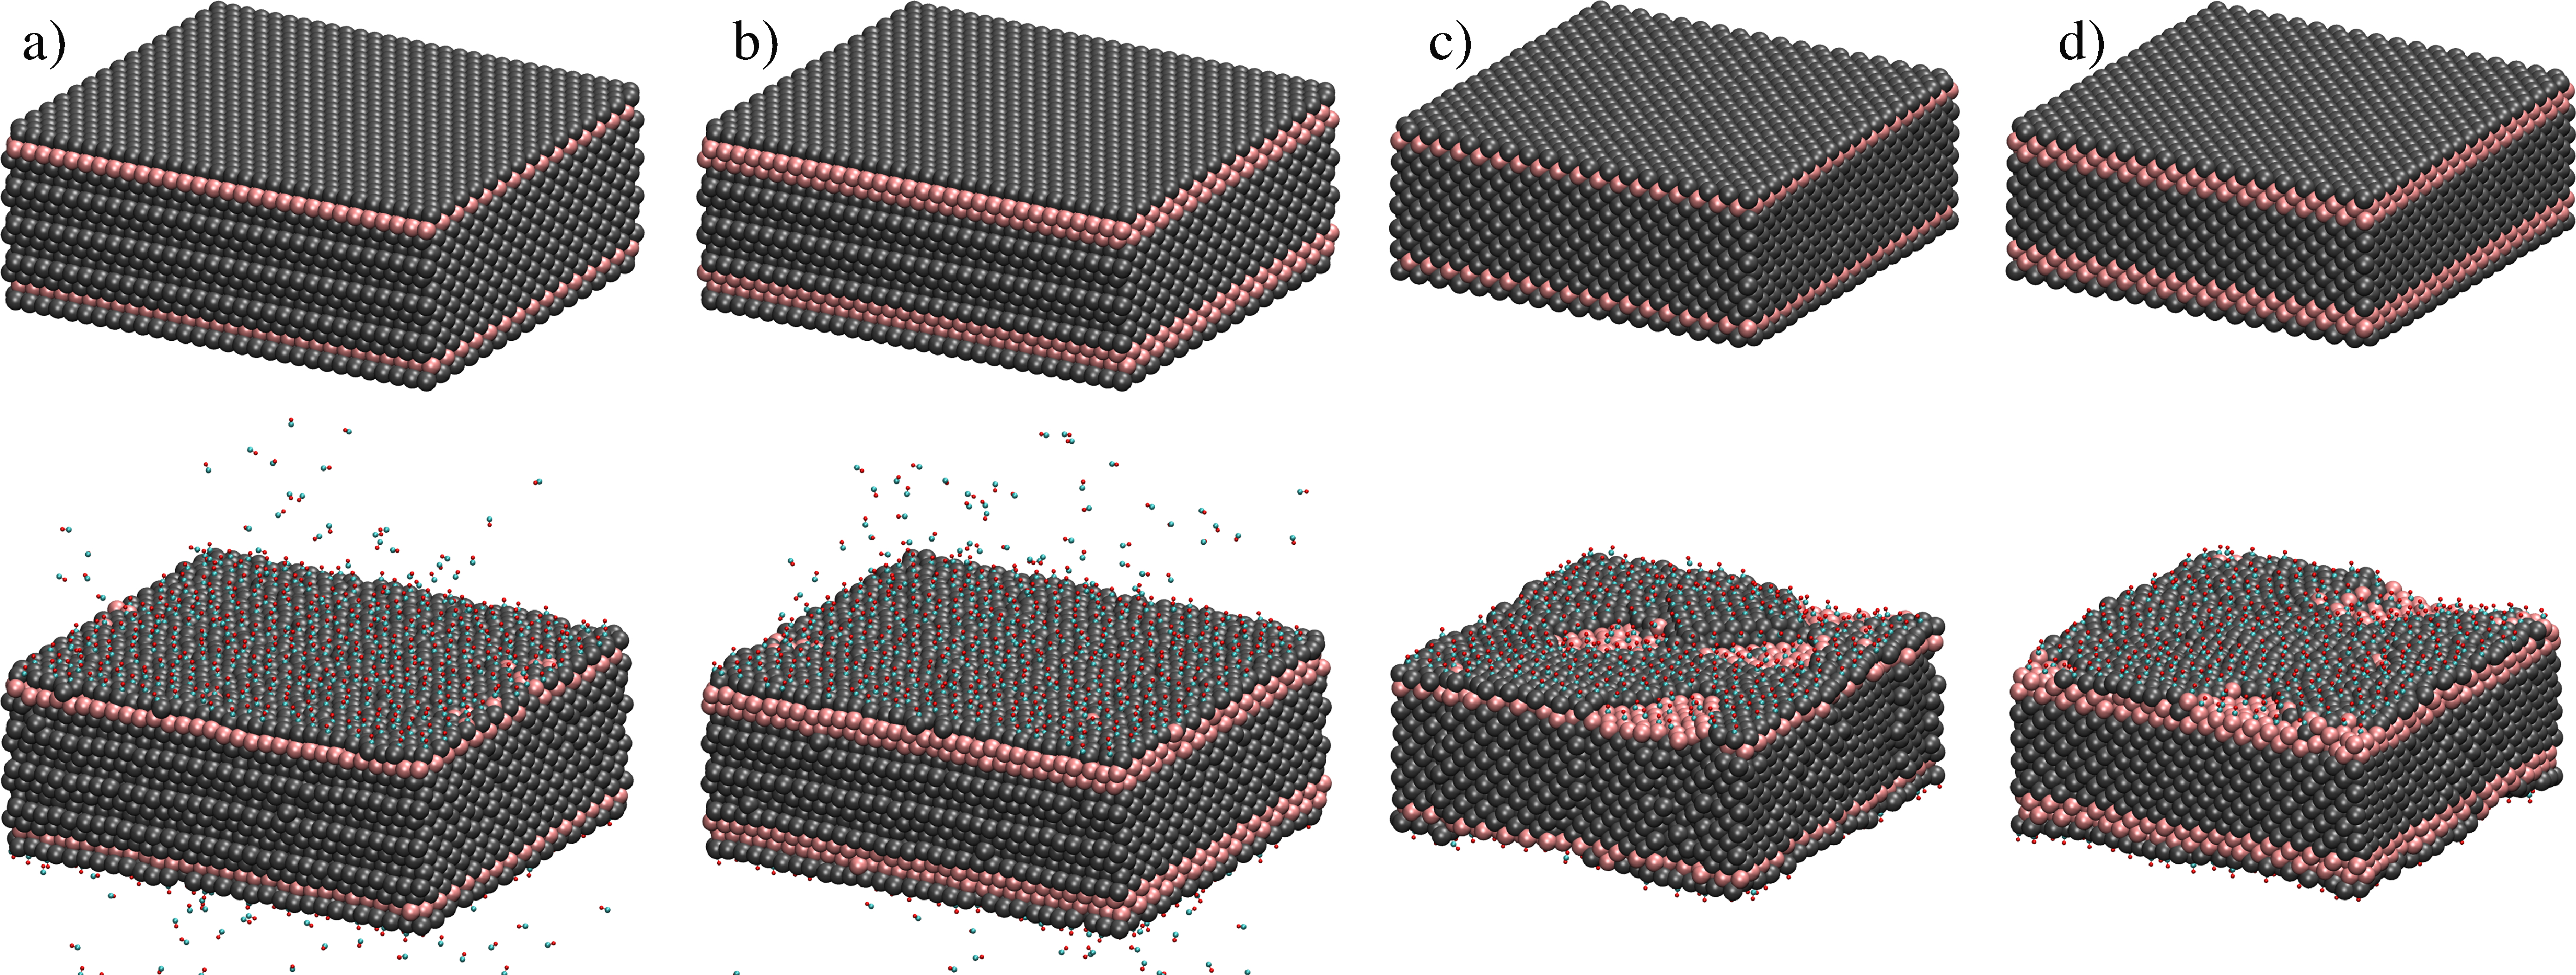
\includegraphics[width=0.8\linewidth]{../figures/appC/systems.pdf}
  \caption{\ce{Pt} atoms are colored gray while \ce{Pd} are colored pink. The
top row depicts near surface alloys with a sandwiched Pt (surface), Pd
(subsurface), Pt (bulk) system before significant warming. Systems (a) and (b)
display the low-energy (111) facets and only differ with number of layers of Pd
with (a) having one layer and (b) having two layers. Systems (c) and (d)
display the (100) facets on the surface and also are only different with regard
to the number of Pd layers, one and two respectively.}
\label{fig:biSystems}
\end{figure}
\end{landscape}

\subsection{System Details}
The systems were constructed from a FCC \ce{Pt} crystal that was ``sliced'' to
display either a (111) or (100) facet in the {\em z}-direction while being
periodic in the {\em x} and {\em y} directions. The bulk of the crystal was
kept as \ce{Pt} while one or two layers directly underneath the surface were
converted to \ce{Pd}. The ideal systems are highlighted in the top row of
Figure \ref{fig:biSystems}. The (111) systems have dimensions of
$71.41\times82.44\times100$ while the (100) systems are
$68.78\times68.78\times100$. \ce{Pd} was chosen as the subsurface layer because
of its stronger binding to \ce{CO}. During preliminary simulations, a variety
of possible systems that switched the order of the metals or the number of
layers at the surface or beneath the surface and the presence of \ce{Pd} on the
surface led to no reconstruction because there was a lack of any driving force.
When \ce{Pt} is on the surface, there are two effects that could lead to
restructuring, \ce{Pt}'s higher surface energy, {\em i.e.} desire to be in a
bulk environment, and the greater strength of the \ce{Pd\bond{-}CO} compared to
the \ce{Pt\bond{-}CO} interaction.

The systems were initially equilibrated at ?~K over a period of ? ns, after
which they were dosed with enough Carbon Monoxide (CO) to correspond to 0,
0.25, or 0.5 monolayers (ML) of coverage. The systems were further equilibrated
in the canonical (NVT) ensemble at ?~K before switching to the microcanonical
(NVE) ensemble for data collection. 

\section{Results \& Discussion}
The (100) surfaces were inherently unstable at any CO-coverage and the surface
\ce{Pt} collapsed to domains of (111) which exposed the underlying (100)
\ce{Pd} which did remain fairly stable. As shown in figure
\ref{fig:biSystems}.c and \ref{fig:biSystems}.d the initially (100) surface
restructures to the lower energy (111) domains. Additionally, because of the
way adsorbate coverage was initially calculated, this restructuring creates
more surface sites for the \ce{CO} to bind too which can be seen by comparing
the (111) to the (100) systems and seeing the large amount of \ce{CO} that is
not adsorbed in the (111) systems.


\section{Summary}
